\documentclass{article}

% if you need to pass options to natbib, use, e.g.:
\PassOptionsToPackage{numbers,compress}{natbib}
% before loading neurips_2026

\usepackage[final,main]{neurips_2026}
\makeatletter
\renewcommand{\@noticestring}{}
\makeatother

\usepackage[utf8]{inputenc}
\usepackage[T1]{fontenc}
\usepackage{hyperref}
\usepackage{url}
\usepackage{booktabs}
\usepackage{amsfonts}
\usepackage{nicefrac}
\usepackage{microtype}
\usepackage{xcolor}
\usepackage{graphicx}
\usepackage{amsmath}

\title{Implementing and Analyzing a Fine-Grained Hallucination Mitigation Pipeline for Large Vision-Language Models}

\author{%
  Abdulaziz Alqahtani \quad Alwaleed Alharthi\\[4pt]
  Supervisor: Dr. Muzammil Behzad\\[4pt]
  King Fahd University of Petroleum and Minerals\\
}

\begin{document}

\maketitle

\begin{abstract}
Large vision-language models (LVLMs) can generate fluent answers that contain visually unsupported objects, attributes, or relations. This hallucination problem is difficult to mitigate with coarse response-level labels because a single response may contain both grounded and ungrounded statements with different severities. In this work, we implement and analyze a fine-grained hallucination mitigation pipeline that converts released hallucination supervision into structured critiques, uses those critiques for rewrite-based preference construction, validates preference pairs with LVLM judges, repairs weak pairs with LLaVA, and trains LLaVA adapters with DPO-style objectives. We compare a base LLaVA model, standard DPO, direct HSA-DPO, a zero-shot judged severity-margin HSA-DPO-M variant, and a two-shot judged severity-margin HSA-DPO-M variant. The results are mixed but informative: POPE adversarial F1 remains slightly higher for the base model ($84.18$) than for the completed trained variants with valid POPE F1 values ($83.87$--$83.91$), while Object HalBench and AMBER hallucination metrics improve substantially after alignment. In particular, Object HalBench CHAIRs decreases from $53.00$ to $36.00$ for the zero-shot judged severity-margin variant and to $40.33$ for the two-shot judged variant; AMBER-Hal decreases from $35.90$ to $25.50$ and $26.90$, respectively. These findings suggest that fine-grained critique and severity-aware preference training are useful for reducing generative hallucination, but their benefits are benchmark-dependent and do not automatically transfer to every hallucination evaluation setting.
\end{abstract}

\section{Introduction}

Large vision-language models (LVLMs) have become a standard foundation for multimodal assistants, image-grounded dialogue systems, and open-ended visual reasoning. Recent systems connect strong visual encoders with large language models through lightweight modality bridges, visual instruction tuning, or instruction-aware visual feature extraction, enabling models such as BLIP-2, LLaVA, and InstructBLIP to answer open-ended image questions and follow multimodal instructions \citep{li2023blip2,liu2023visual,dai2023instructblip}. Their ability to produce fluent natural-language responses from visual inputs has improved rapidly, but this fluency can obscure a persistent reliability problem: models often describe objects, attributes, spatial relations, events, or implications that are not supported by the image. This phenomenon, commonly discussed as hallucination, is especially consequential for LVLMs because users frequently rely on generated text as a faithful account of visual evidence \citep{liu2024survey,rohrbach2018object}. A response that is linguistically plausible but visually ungrounded can degrade trust, mislead downstream decision making, and make model behavior difficult to audit.

Prior work has approached LVLM hallucination from both evaluation and mitigation perspectives. Evaluation studies have shown that hallucination is not a single uniform failure mode: unsupported object mentions, incorrect attributes, and erroneous relationships can arise for different reasons and may require different corrective signals \citep{rohrbach2018object,gunjal2024detecting,chen2024unified}. Mitigation work has explored robust instruction tuning, decoding-time interventions, preference distillation, and reinforcement or preference learning from human or AI feedback \citep{liu2024robust,zhou2024analyzing,li2023silkie,yu2024rlhfv}. These approaches have improved multimodal faithfulness, but they also expose practical challenges. Coarse response-level labels do not specify what is wrong or how serious the error is. Human preference construction can be expensive. Fully automated preference construction can introduce noisy pairs if a rewritten response is not actually more faithful than the original. As a result, a useful mitigation pipeline must manage not only model optimization, but also supervision granularity, rewrite quality, validation, and severity-aware weighting.

This project implements and analyzes a fine-grained hallucination mitigation pipeline for LVLMs rather than proposing a wholly new LVLM architecture. We build on the released HSA-DPO fine-grained hallucination supervision, which contains both hallucinated and non-hallucinated image-response samples. The pipeline treats hallucination handling as a staged workflow. First, it extracts structured critiques that identify the hallucination type, provide a rationale, and assign a severity score; clean samples are preserved rather than forced into a hallucination category. Second, critiques guide response rewriting with LLaVA, producing a candidate corrected response. For hallucinated samples, the rewritten response is used as the chosen response and the original hallucinated response as the rejected response, with the severity score attached to the pair. Third, preference construction can follow either a direct preference path or a judged preference path, where Gemini or GPT-style judges assess whether the candidate pair is sufficiently reliable. Rejected pairs can be repaired by LLaVA or removed from the training set. Finally, the resulting pairs are used for DPO or HSA-DPO training, where more severe hallucinations receive stronger penalty under the severity-aware objective \citep{rafailov2024dpo,xiao2025hsa}.

The central contribution of this work is therefore an implementation-oriented study of how fine-grained critique signals can be transformed into preference data for hallucination mitigation. This framing is deliberately cautious. We do not claim to introduce a new multimodal backbone, a new benchmark, or a fully novel preference-learning algorithm. Instead, we organize the stages needed to operationalize fine-grained hallucination supervision: critique extraction, critique-conditioned rewriting, preference validation, repair or filtering of weak pairs, and severity-aware training. This organization makes the pipeline easier to inspect and compare against simpler alternatives, including base LLaVA, direct preference training, standard DPO, HSA-DPO, and judged-preference variants.

Our evaluation is designed around hallucination-sensitive benchmarks, including POPE, Object HalBench, and AMBER \citep{li2023pope,rohrbach2018object,wang2023amber}. The resulting picture is mixed rather than uniformly positive. In our experiments, POPE does not show a clear improvement over the base model, suggesting that the pipeline does not automatically improve every binary or object-probing hallucination setting. At the same time, Object HalBench and AMBER hallucination-oriented metrics show improvements, indicating that fine-grained critique and severity-aware preference construction can be useful for generative and object hallucination scenarios. These findings motivate the main argument of the paper: fine-grained hallucination supervision is valuable, but its benefits depend on the evaluation setting, the quality of intermediate preference pairs, and the alignment between training signals and benchmark behavior.

\section{Related Work}

\subsection{Large Vision-Language Models and Instruction Tuning}

The recent progress of LVLMs is closely tied to methods that adapt pretrained language models to visual inputs. BLIP-2 introduced a parameter-efficient strategy that bridges frozen image encoders and frozen language models using a lightweight querying transformer, reducing the cost of vision-language pretraining while preserving strong zero-shot image-to-text capabilities \citep{li2023blip2}. LLaVA extended instruction tuning into the multimodal setting by using GPT-generated language-image instruction data to train an end-to-end visual assistant that connects a vision encoder with a language model \citep{liu2023visual}. InstructBLIP further studied vision-language instruction tuning at scale, converting diverse datasets into instruction format and introducing instruction-aware visual feature extraction to improve zero-shot generalization \citep{dai2023instructblip}. These systems show why LVLMs are attractive for open-ended visual interaction: they inherit the generative flexibility of LLMs while grounding responses in image representations.

At the same time, the same open-ended generation ability that makes LVLMs useful also makes hallucination harder to control. Unlike closed-set recognition models, LVLMs generate free-form text whose visual claims may vary in granularity, certainty, and factual grounding. A single response can mix correct visual observations with unsupported details, making response-level supervision too coarse for mitigation. This motivates the fine-grained framing adopted in our project, where hallucinations are decomposed by type, rationale, and severity before being transformed into preference data.

\subsection{LVLM Hallucination and Evaluation}

Hallucination in vision-language generation predates the recent wave of instruction-tuned LVLMs. In image captioning, object hallucination was identified as a failure mode in which generated captions mention objects that are absent from the image, often due to language priors, dataset bias, or weak visual grounding \citep{rohrbach2018object}. Modern LVLMs extend this problem to longer and more interactive outputs. Because they can produce detailed explanations, descriptions, and multi-turn answers, hallucinations may appear not only as nonexistent objects but also as incorrect attributes, counts, actions, spatial relations, and causal interpretations \citep{liu2024survey}. This broader output space makes evaluation more difficult than checking whether a short caption contains a small set of object words.

Recent hallucination evaluation work has therefore moved toward more systematic detection protocols and benchmark suites. Model-based and benchmark-based methods aim to identify whether a response is visually supported, sometimes by using stronger evaluators or specialized prompts \citep{gunjal2024detecting,chen2024unified}. POPE evaluates object hallucination through polling-style object-presence questions, while AMBER provides a multi-dimensional and LLM-free benchmark for hallucination evaluation \citep{li2023pope,wang2023amber}. Object HalBench and CHAIR-style measurements trace back to the broader object hallucination literature, where the key question is whether generated object mentions are grounded in the image \citep{rohrbach2018object}. HallusionBench adds another diagnostic perspective by evaluating entangled language hallucination and visual illusion in image-context reasoning tasks \citep{guan2024hallusionbench}. These benchmarks are complementary rather than interchangeable: a method that improves long-form generation may not necessarily improve binary object-presence decisions, and a method optimized for object errors may not address attribute or relationship hallucinations. This distinction is important for our analysis because our pipeline targets fine-grained critique and rewriting, so its expected gains are strongest when the evaluation rewards faithful generation rather than only response-level yes/no behavior.

The evaluation literature also motivates a more structured definition of hallucination. A single binary label indicating that a response is hallucinated can be useful for aggregate scoring, but it is insufficient for training a model to avoid specific errors. Fine-grained supervision can identify whether an error concerns an object, an attribute, or a relationship, and it can explain why the response is unsupported by the image. Such structure is valuable for building corrective data because a rewriting model can use the critique to remove or revise the unsupported content rather than merely learning that the entire response is bad.

\subsection{Hallucination Mitigation and Preference Learning}

Mitigation methods for LVLM hallucination can be broadly grouped into inference-time interventions and training-time alignment. Inference-time approaches attempt to reduce hallucination without updating model weights, for example by modifying decoding behavior, constraining generation, or analyzing internal signals associated with object hallucination \citep{zhou2024analyzing}. These methods are attractive because they can be applied to existing models, but they may have limited ability to reshape the model's underlying preferences across diverse visual contexts. Training-time approaches instead alter the model through instruction tuning, robust data construction, or preference optimization \citep{liu2024robust,li2023silkie,yu2024rlhfv}. Such approaches can produce more persistent behavioral changes, but they require high-quality supervision and careful control of noisy or misleading training examples.

Preference learning has become a particularly influential strategy for aligning generative models with desired behavior. Direct Preference Optimization (DPO) provides a practical objective for learning from chosen/rejected response pairs without explicitly training a separate reward model \citep{rafailov2024dpo}. In the multimodal setting, preference pairs can encode which response is more visually faithful, more helpful, or less hallucinatory. Systems such as Silkie and RLHF-V demonstrate that preference-style supervision can improve LVLM behavior by distilling or collecting feedback that favors grounded responses \citep{li2023silkie,yu2024rlhfv}. However, constructing reliable preference pairs for hallucination mitigation remains difficult. If the chosen response is only superficially better, or if the rejected response contains mild rather than severe hallucination, the optimization signal may be weak or noisy.

Our pipeline follows this preference-learning direction but emphasizes the intermediate data construction problem. The chosen response is not assumed to exist in the raw data; it is generated through critique-guided rewriting. The rejected response is the original hallucinated output when a hallucination is present. The quality of the pair can then be checked through direct rules or judged preference validation, and weak pairs may be repaired or discarded. This design reflects a practical observation: DPO-style objectives are only as useful as the preference data they consume, so a hallucination mitigation pipeline must include mechanisms for producing, checking, and filtering those preferences before optimization.

\subsection{Fine-Grained Feedback and Severity-Aware Training}

Fine-grained feedback offers a way to bridge detection and mitigation. Rather than labeling an entire response as acceptable or unacceptable, fine-grained feedback identifies localized problems and provides additional information about the nature of the error. For LVLM hallucination, this can include the hallucination category, a textual rationale, and a severity score. Such feedback is useful because hallucinations differ in both type and consequence. A minor attribute mismatch and a fabricated object central to the answer should not necessarily contribute the same training signal. Treating them equally can underweight serious failures and overweight small imperfections.

HSA-DPO is closely related to this view because it incorporates hallucination severity into preference optimization \citep{xiao2025hsa}. The core idea is to make the penalty stronger when the rejected response contains more severe hallucination, while retaining the efficiency of a DPO-style objective \citep{rafailov2024dpo}. This creates a direct connection between fine-grained critique extraction and model training: critiques are not only diagnostic artifacts, but also inputs to the construction and weighting of preference pairs. Severity-aware training is therefore especially relevant when the dataset contains heterogeneous hallucination examples with different levels of visual inconsistency.

The present project is an implementation and analysis of this fine-grained, severity-aware paradigm. We use released HSA-DPO supervision as the data source, preserve non-hallucinated samples, extract structured critiques for hallucinated samples, and convert those critiques into rewrite-based preference data. We also include judged-preference variants in which Gemini or GPT-style evaluators assess candidate pairs, allowing the pipeline to remove or repair examples that may otherwise introduce noise. This places our work between benchmark-level hallucination analysis and full model alignment: it studies the engineering path from fine-grained hallucination labels to preference data and then to DPO or HSA-DPO training, while evaluating the resulting behavior cautiously across POPE, Object HalBench, and AMBER.

\section{Methodology}

The methodological problem is defined as follows. Given an image-question or image-instruction input $x$ and an original LVLM response $\hat{y}$, the objective is to construct or select a better response $y^+$ that is more visually grounded in the image. The improved response should remove unsupported visual claims while preserving correct visual details from the original response. In preference-learning terms, the project transforms hallucination supervision into reliable triples $(x, y^+, y^-)$, where $y^-$ is the hallucinated or weaker response and $y^+$ is the preferred grounded response. This formulation motivates three research questions: \textbf{RQ1:} Can released fine-grained hallucination annotations be converted into structured critique records that support preference construction? \textbf{RQ2:} Can judged preference validation and repair improve the quality of preference pairs used for alignment? \textbf{RQ3:} Does severity-aware DPO reduce hallucination compared with the base LLaVA model, standard DPO, and direct HSA-DPO?

Our methodology treats hallucination mitigation as a data construction and preference-alignment problem rather than only a model-training problem. The pipeline begins with released fine-grained hallucination supervision, converts it into normalized critique records, constructs or reuses preference pairs, validates, repairs, and re-verifies weak pairs when needed, and finally trains LVLM adapters with DPO-style objectives. Figure~\ref{fig:pipeline} summarizes the resulting five-stage workflow. The design has two goals. First, it preserves the fine-grained supervision signal: hallucination type, rationale, evidence text, and severity are retained instead of being collapsed into a single binary label. Second, it separates two preference-data paths: a direct path that trains on the released preference pairs as provided, and a judged path that uses Gemini/GPT checks plus LLaVA repair to reduce noisy or weak pairs before training.

\begin{figure}[t]
  \centering
  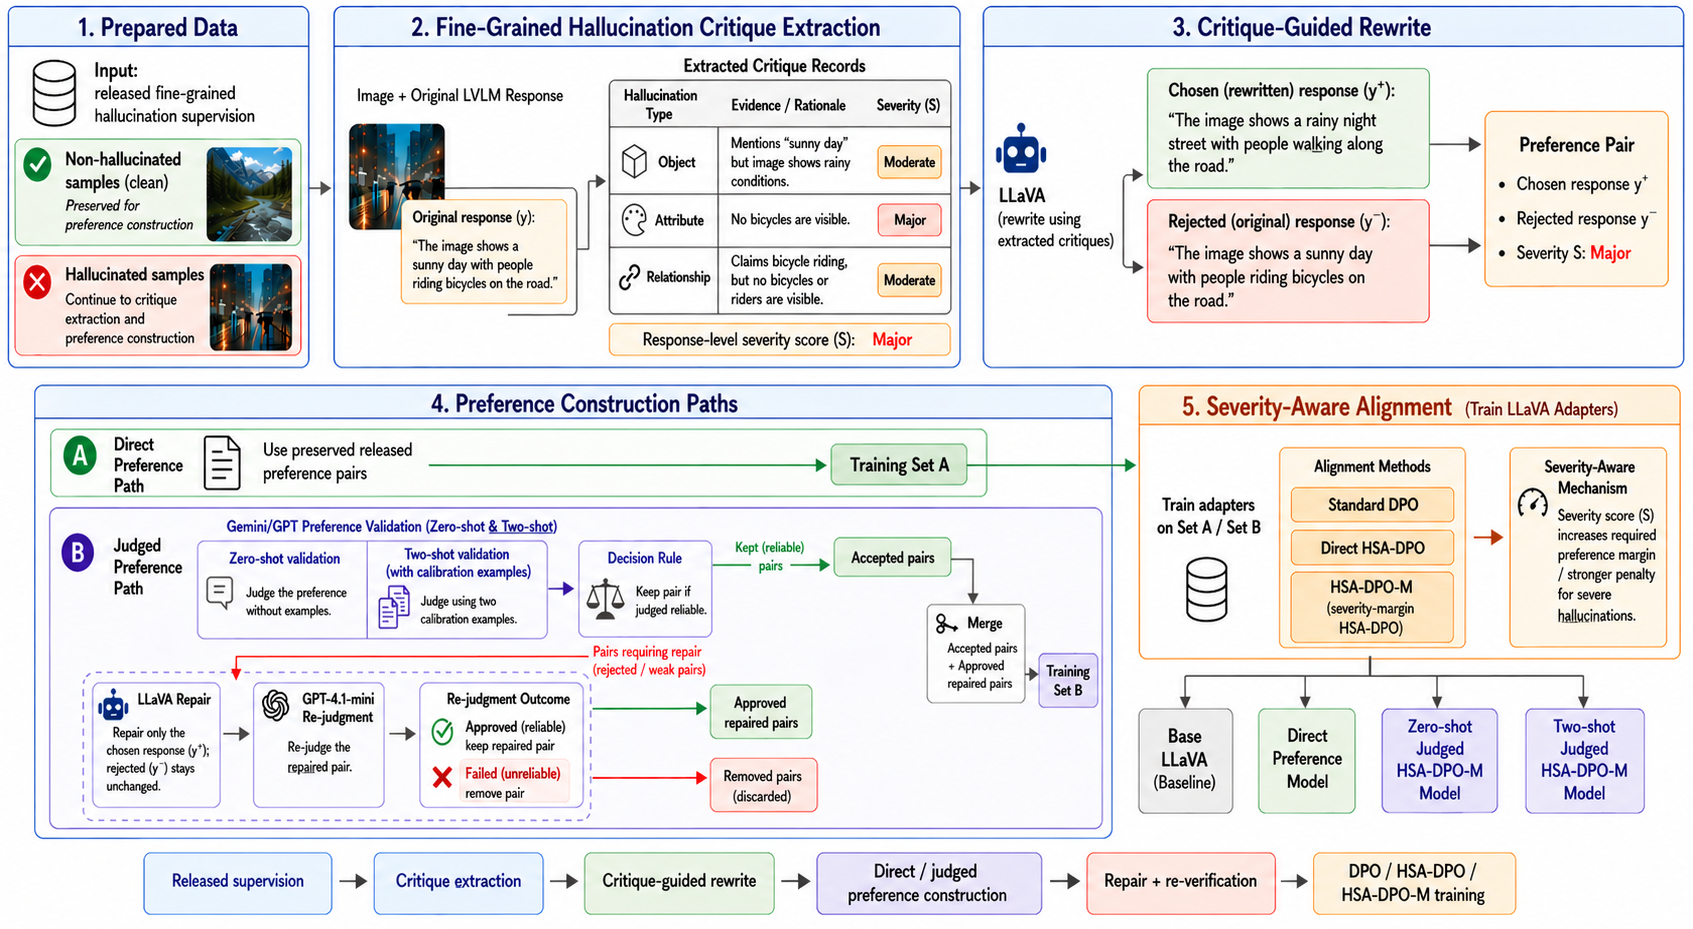
\includegraphics[width=\linewidth]{../diagram_overview.png}
  \caption{Overview of the implemented fine-grained hallucination mitigation pipeline. Released supervision is normalized into critique records, LLaVA is used for critique-guided rewriting or repair, preference pairs are routed through direct and judged paths, weak repaired pairs are re-verified, and the resulting training sets are used for DPO/HSA-DPO style severity-aware alignment. Evaluation is reported separately in Section~\ref{sec:results}.}
  \label{fig:pipeline}
\end{figure}

\subsection{Problem Formulation and Notation}

Let $I_i$ denote an image and $x_i$ denote the associated text input or image-grounded instruction. A candidate LVLM response is denoted by $\hat{y}_i$. The goal is to train a policy LVLM $\pi_\theta$ that prefers image-grounded responses over hallucinated ones. For hallucination supervision, we use a fine-grained feedback representation rather than a response-level label. For each response, the critique set is
\begin{equation}
H_i = \{h_i^j\}_{j=1}^{T_i},
\end{equation}
where each critique item $h_i^j$ contains a hallucination type, rationale, evidence span, severity label, and severity score. In our implementation, hallucination types are normalized into object, attribute, and relationship categories when available. The corresponding response-level severity score is computed as an average over available sentence- or span-level severity scores:
\begin{equation}
S_i = \frac{1}{T_i}\sum_{j=1}^{T_i} s_i^j ,
\end{equation}
where $s_i^j$ is the severity score for critique $h_i^j$. If a sample is non-hallucinated, it is preserved as a clean supervision example and does not enter the rewrite-repair branch.

For preference optimization, each training example is represented as
\begin{equation}
p_i = (I_i, x_i, y_i^+, y_i^-, S_i),
\end{equation}
where $y_i^+$ is the chosen response, $y_i^-$ is the rejected response, and $S_i$ is the hallucination severity associated with the rejected response. In the mitigation setting, the rejected response is typically the original hallucinated response, while the chosen response is a corrected rewrite or a released preferred response.

\subsection{Fine-Grained Hallucination Critique Extraction}

The first stage constructs a normalized fine-grained feedback dataset from the released hallucination supervision. The raw detection-side data contains both hallucinated and non-hallucinated image-response samples. For each row, the parser extracts the assessed response text, the raw annotation text, hallucination tags, hallucination rationales, and severity information. The output is a normalized dataset
\begin{equation}
D_{\mathrm{FAIF}} = \{(I_i, x_i, \hat{y}_i, H_i, S_i, m_i)\}_{i=1}^{N},
\end{equation}
where $m_i$ stores metadata such as the annotation source and the original raw annotation string. This metadata is important because it allows later stages to audit how a critique was obtained, rather than only seeing the normalized field values.

This stage does not regenerate all annotations with a new hosted model. Instead, the released fine-grained supervision is treated as the primary supervision source. This choice keeps the pipeline closer to the available data and avoids turning the method into a costly relabeling process. However, the implementation also stores appendix-aligned prompt templates for reproducibility, so that future work can regenerate or extend the fine-grained feedback when stronger evaluators or additional annotation budgets are available.

Clean samples are handled explicitly. If the released annotation indicates that no hallucination is present, the row is stored with an empty critique list and a non-hallucinated flag. These clean rows are not forced into the rewrite stage. This prevents the pipeline from constructing artificial preference pairs for responses that do not require mitigation.

\subsection{Detector-Style Dataset Construction}

After critique extraction, the normalized records are converted into a detector-style supervised fine-tuning format. This stage is included for reproducibility and analysis: it shows how fine-grained feedback can be transformed into a training set for a local hallucination detector, even though our final time-constrained experiments rely primarily on released preference pairs for alignment training. The human turn contains the image marker, the image-grounded question or context, and the candidate response to be assessed. The assistant target contains either a structured hallucination report or a normalized no-hallucination target.

For hallucinated rows, the target includes the hallucination tags and severity scores. For clean rows, the target is a compact no-hallucination response. This format keeps hallucinated and non-hallucinated examples in the same training representation, which is necessary for a detector to learn both when to flag unsupported content and when to leave a grounded response unchanged. We preserve deterministic ordering and sampling rules so the generated detector dataset is reproducible.

\subsection{Critique-Guided Rewrite and Preference Pair Construction}

The rewrite component maps a hallucinated response and its critique set into a corrected response. Formally, a rewriting model $M_{\mathrm{wri}}$ receives the image, question, original response, and critique set:
\begin{equation}
y_i' = M_{\mathrm{wri}}(I_i, x_i, \hat{y}_i, H_i).
\end{equation}
The intended role of this stage is not to produce a completely new answer from scratch, but to revise the original response using the critique as targeted guidance. The prompt instructs the model to remove unsupported claims, preserve correct image-grounded details, and avoid introducing new visual assumptions.

The resulting preference pair is formed as
\begin{equation}
y_i^+ = y_i', \qquad y_i^- = \hat{y}_i.
\end{equation}
The severity score $S_i$ is attached to the pair so that downstream DPO variants can weight or margin the rejected response according to hallucination severity. The implementation filters obvious failure cases, including empty rewrites, missing images, and rewrites that are identical to the rejected response.

In the final experimental organization, we also use the released preference dataset directly. This gives the project two complementary data sources: critique-derived records for interpretability and reproducibility, and released chosen/rejected preference pairs for scalable DPO training. The released preference pairs are important because they provide thousands of ready-to-train examples, whereas fully regenerating all chosen responses locally is slower and more compute-intensive.

\subsection{Preference Validation and Repair}

Preference quality is a central source of risk in automatic hallucination mitigation. A pair is useful only if the chosen response is actually more visually grounded than the rejected response. If a chosen response removes useful detail, adds a new unsupported claim, or fails to correct the original hallucination, then DPO training may learn from noisy supervision. To address this issue, the project supports two preference paths.

\paragraph{Direct preference path.}
The direct path uses the released preference data without additional API judging. This path preserves the original chosen/rejected pairs and severity scores and is used to train a direct HSA-DPO model and a matched standard DPO baseline. The purpose of this path is to establish a clean baseline: if the released preference dataset already contains useful alignment signal, then direct DPO/HSA-DPO training should be a strong and simple reference point.

\paragraph{Judged preference path.}
The judged path applies hosted LVLM judges to evaluate whether the chosen response should be accepted. For a preference pair $p_i$, each judge produces a binary decision and a short reason:
\begin{equation}
v_i^k = (\mathrm{approved}_i^k, r_i^k),
\end{equation}
where $k$ indexes the judge family. The implementation supports Gemini-only, OpenAI-only, or Gemini+OpenAI checking. The final acceptance decision is configurable: a permissive setting can keep a pair if either judge approves, while a stricter setting can require both judges to approve. All votes and reasons are stored in metadata so the decision remains auditable.

Pairs rejected by the judged path are not automatically discarded. They are routed to a repair stage in which LLaVA receives the original rejected response, the current chosen response, severity information, and the judge feedback. LLaVA then produces a repaired chosen response while the rejected response remains fixed. The repaired pair is re-verified by the judge, and only approved repaired pairs are merged with initially accepted pairs to form the judged-preference training set. Failed repaired pairs are removed. This design separates diagnosis from repair: Gemini/GPT are used as quality checkers, while LLaVA remains the local model used to produce repaired training text.

\subsection{Training Sets}

The pipeline therefore produces two primary training sets. Training Set A is the direct preference set:
\begin{equation}
D_A = D_{\mathrm{pref}}^{\mathrm{released}},
\end{equation}
where released preference pairs are used directly. Training Set B is the judged-preference set:
\begin{equation}
D_B = D_{\mathrm{accepted}} \cup D_{\mathrm{approved}\text{-}\mathrm{repaired}},
\end{equation}
where $D_{\mathrm{accepted}}$ contains initially judge-approved pairs and $D_{\mathrm{approved}\text{-}\mathrm{repaired}}$ contains only repaired pairs that pass the re-verification step. These two training sets allow the project to compare whether extra preference quality control helps or whether direct training on released preferences is already sufficient.

\subsection{Severity-Aware Preference Optimization}

The final alignment stage trains LLaVA adapters using DPO-style objectives. Standard DPO optimizes the policy to prefer the chosen response over the rejected response relative to a reference model:
\begin{align}
\Delta_i &=
\left[\log \pi_\theta(y_i^+|I_i,x_i)-\log \pi_\theta(y_i^-|I_i,x_i)\right] \nonumber\\
&\quad -
\left[\log \pi_{\mathrm{ref}}(y_i^+|I_i,x_i)-\log \pi_{\mathrm{ref}}(y_i^-|I_i,x_i)\right], \\
\mathcal{L}_{\mathrm{DPO}} &=
-\mathbb{E}_{p_i}
\left[
\log \sigma\left(
\beta \Delta_i
\right)
\right],
\end{align}
where $\pi_\theta$ is the trained policy, $\pi_{\mathrm{ref}}$ is the reference model, and $\beta$ controls the preference sharpness \citep{rafailov2024dpo}.

We train three relevant variants. The first is standard DPO, which ignores severity and treats all preference pairs equally. The second is HSA-DPO-style severity weighting, where the rejected response log-probability term can be weighted by the rejected response severity score. This follows the intuition that a severe hallucinated response should be penalized more strongly than a mild one \citep{xiao2025hsa}. The third is our severity-margin variant. In this variant, severity does not directly multiply the log-probability terms; instead, it increases the required margin between the chosen and rejected responses:
\begin{equation}
\mathcal{L}_{\mathrm{margin}} =
-\mathbb{E}_{p_i}
\left[
\log \sigma\left(
\beta\left(\Delta_i - \lambda \frac{S_i}{S_{\max}}\right)
\right)
\right],
\end{equation}
where $\Delta_i$ is the DPO log-ratio difference between the policy and reference model, $S_{\max}$ is the maximum normalized severity score, and $\lambda$ is the severity-margin scale. Higher severity therefore requires the policy to create a larger preference gap in favor of the chosen response.

This training design allows us to compare whether hallucination severity is more useful as a direct weight or as a required preference margin. It also allows a matched comparison with standard DPO, where severity information is ignored.

\subsection{Implementation Workflow Support}

The implementation is organized to make the full workflow reproducible and inspectable. Each processing step writes JSONL artifacts and a statistics file. The critique-extraction scripts write normalized fine-grained critique records, the detector-construction scripts write detector-style examples, the released-preference validation scripts write accepted pairs, rejected pairs, and audit records containing judge decisions, the repair scripts write repaired candidates, and the repair-verification scripts write approved repairs, failed repairs, and the final verified preference dataset. The alignment scripts then write LoRA adapters and trainer states for the trained models.

The current repository provides separate scripts for the direct and judged paths. The direct path trains from the released preference file and supports both HSA-DPO and standard DPO. The judged path first validates released pairs, repairs rejected rows, re-verifies repaired rows, and then trains on the merged accepted/approved-repaired preference dataset. Evaluation is kept separate from training and is reported through automatic benchmark summaries, with paper-comparable and supplemental local results separated to avoid overstating conclusions.

\section{Experiments}

We evaluated the proposed mitigation pipeline using a controlled comparison built around LLaVA-1.5-7B as the base large vision-language model. The released fine-grained hallucination supervision was first normalized into $16{,}143$ feedback records, consisting of $7{,}643$ hallucinated samples and $8{,}500$ non-hallucinated samples, and the main alignment experiments used $8{,}386$ released image-response preference pairs. We compared the unaligned LLaVA-1.5-7B model, a standard DPO model trained on the same preference source, a direct severity-aware HSA-DPO model, a zero-shot judged severity-margin HSA-DPO-M model, and a two-shot judged severity-margin HSA-DPO-M model. In both judged runs, initial preference validation used Gemini-2.5-Flash-Lite and GPT-4o-mini with an ``either judge approves'' rule, rejected or weak pairs were repaired with LLaVA-1.5-7B, and repaired pairs were re-verified with GPT-4.1-mini. The zero-shot path presented each target pair directly after the validation rubric, while the two-shot path inserted two calibration examples into the Gemini/GPT validation and GPT-4.1-mini re-verification prompts. To ensure a fair comparison, all reported DPO/HSA-DPO runs used the same training budget and optimization settings unless otherwise stated: one training epoch, per-device batch size $1$, effective batch size $32$, learning rate $2\times10^{-6}$, DPO temperature parameter $\beta=0.1$, LoRA rank $128$, LoRA scaling factor $256$, maximum sequence length $1024$, cosine learning-rate scheduling, no warmup, and zero weight decay. The severity-margin HSA-DPO-M objective used a severity margin scale of $0.5$. Adapter training was run on a rented VastAI instance with an NVIDIA RTX 6000 Ada Generation GPU with 48 GB VRAM. Model behavior was evaluated using hallucination-oriented benchmarks including POPE, Object HalBench, and AMBER, with the analysis focusing on precision, recall, F1 score, and hallucination-related error rates rather than claiming uniform improvement across all benchmarks.

\begin{table}[t]
  \centering
  \caption{Judged-preference construction statistics for the zero-shot and two-shot HSA-DPO-M paths. Initial validation checks released preference pairs, LLaVA repairs rejected pairs, and GPT-4.1-mini re-verifies repaired pairs before final training.}
  \label{tab:pipeline-stats}
  \small
  \resizebox{\linewidth}{!}{%
  \begin{tabular}{lrrrrrrr}
    \toprule
    Path & Source pairs & Initially accepted & Initially rejected & Repaired & Approved repairs & Final verified & Train-ready \\
    \midrule
    Zero-shot judged path & 8{,}386 & 7{,}818 & 568 & 473 & 244 & 8{,}062 & 8{,}062 \\
    Two-shot judged path & 8{,}386 & 7{,}132 & 1{,}254 & 1{,}063 & 746 & 7{,}878 & 7{,}874 \\
    \bottomrule
  \end{tabular}%
  }
\end{table}

\section{Results}
\label{sec:results}

Table~\ref{tab:pope-results} reports POPE adversarial results for the completed runs with valid F1 and recall values. On this binary object-presence benchmark, alignment does not improve the main F1 score. The base LLaVA model obtains the highest completed F1 score, $84.18$, while direct HSA-DPO reaches $83.91$, standard DPO reaches $83.88$, and the zero-shot judged severity-margin HSA-DPO-M variant reaches $83.87$. The trained variants with valid POPE results increase precision relative to the base model, with direct HSA-DPO reaching $90.70$ precision compared with $89.92$ for the base model. However, this precision gain is offset by lower recall: the base model obtains $79.13$ recall, while the trained variants remain around $78.07$--$78.33$. The two-shot POPE artifact did not contain valid recall/F1 fields, so it is omitted from this POPE table and figure rather than treated as a comparable F1 result.

\begin{table}[t]
  \centering
  \caption{POPE adversarial results. Accuracy, precision, recall, and F1 are reported as percentages; higher values are better.}
  \label{tab:pope-results}
  \small
  \begin{tabular}{lrrrr}
    \toprule
    Model & Accuracy & Precision & Recall & F1 \\
    \midrule
    LLaVA-1.5-7B & 85.13 & 89.92 & 79.13 & 84.18 \\
    Standard DPO & 85.00 & 90.63 & 78.07 & 83.88 \\
    Direct HSA-DPO & 85.03 & 90.70 & 78.07 & 83.91 \\
    Judged margin HSA-DPO-M (zero-shot) & 84.93 & 90.25 & 78.33 & 83.87 \\
    \bottomrule
  \end{tabular}
\end{table}

Table~\ref{tab:hallucination-results} reports Object HalBench and AMBER hallucination-oriented metrics. These results show a clearer benefit from the mitigation pipeline. On Object HalBench, all trained variants reduce hallucination rates substantially. CHAIRs decreases from $53.00$ for the base model to $38.00$ for direct HSA-DPO, $37.67$ for standard DPO, $36.00$ for zero-shot judged severity-margin HSA-DPO-M, and $40.33$ for the two-shot judged severity-margin HSA-DPO-M run. CHAIRi follows the same overall trend, decreasing from $15.72$ to $11.74$, $11.98$, $10.41$, and $12.81$, respectively. The zero-shot judged severity-margin variant therefore gives the strongest Object HalBench result among the completed runs, while the two-shot run still improves over the base model but does not surpass the zero-shot judged path.

AMBER shows a similar improvement on hallucination-related metrics. AMBER-CHAIR decreases from $7.70$ for the base model to $5.50$ for direct HSA-DPO, $5.20$ for standard DPO, $5.30$ for zero-shot judged severity-margin HSA-DPO-M, and $5.60$ for two-shot judged severity-margin HSA-DPO-M. AMBER-Hal decreases from $35.90$ to $25.10$, $25.20$, $25.50$, and $26.90$, respectively. AMBER-Cog also decreases from $4.30$ to $2.50$--$2.70$ after training. The main tradeoff is AMBER-Cover, which decreases from $51.70$ for the base model to approximately $49.60$--$50.40$ after training. This suggests that the aligned models reduce unsupported content, but may also become slightly more conservative in the amount of visual detail they include.

\begin{table}[t]
  \centering
  \caption{Supplemental local Object HalBench and AMBER hallucination metrics. Lower is better for CHAIRs, CHAIRi, AMBER-CHAIR, AMBER-Hal, and AMBER-Cog; higher is better for AMBER-Cover.}
  \label{tab:hallucination-results}
  \small
  \resizebox{\linewidth}{!}{%
  \begin{tabular}{lrrrrrr}
    \toprule
    Model & CHAIRs & CHAIRi & AMBER-CHAIR & AMBER-Hal & AMBER-Cog & AMBER-Cover \\
    \midrule
    LLaVA-1.5-7B & 53.00 & 15.72 & 7.70 & 35.90 & 4.30 & 51.70 \\
    Standard DPO & 37.67 & 11.98 & 5.20 & 25.20 & 2.50 & 49.90 \\
    Direct HSA-DPO & 38.00 & 11.74 & 5.50 & 25.10 & 2.50 & 50.00 \\
    Judged margin HSA-DPO-M (zero-shot) & 36.00 & 10.41 & 5.30 & 25.50 & 2.50 & 49.60 \\
    Judged margin HSA-DPO-M (two-shot) & 40.33 & 12.81 & 5.60 & 26.90 & 2.70 & 50.40 \\
    \bottomrule
  \end{tabular}%
  }
\end{table}

\begin{figure}[t]
  \centering
  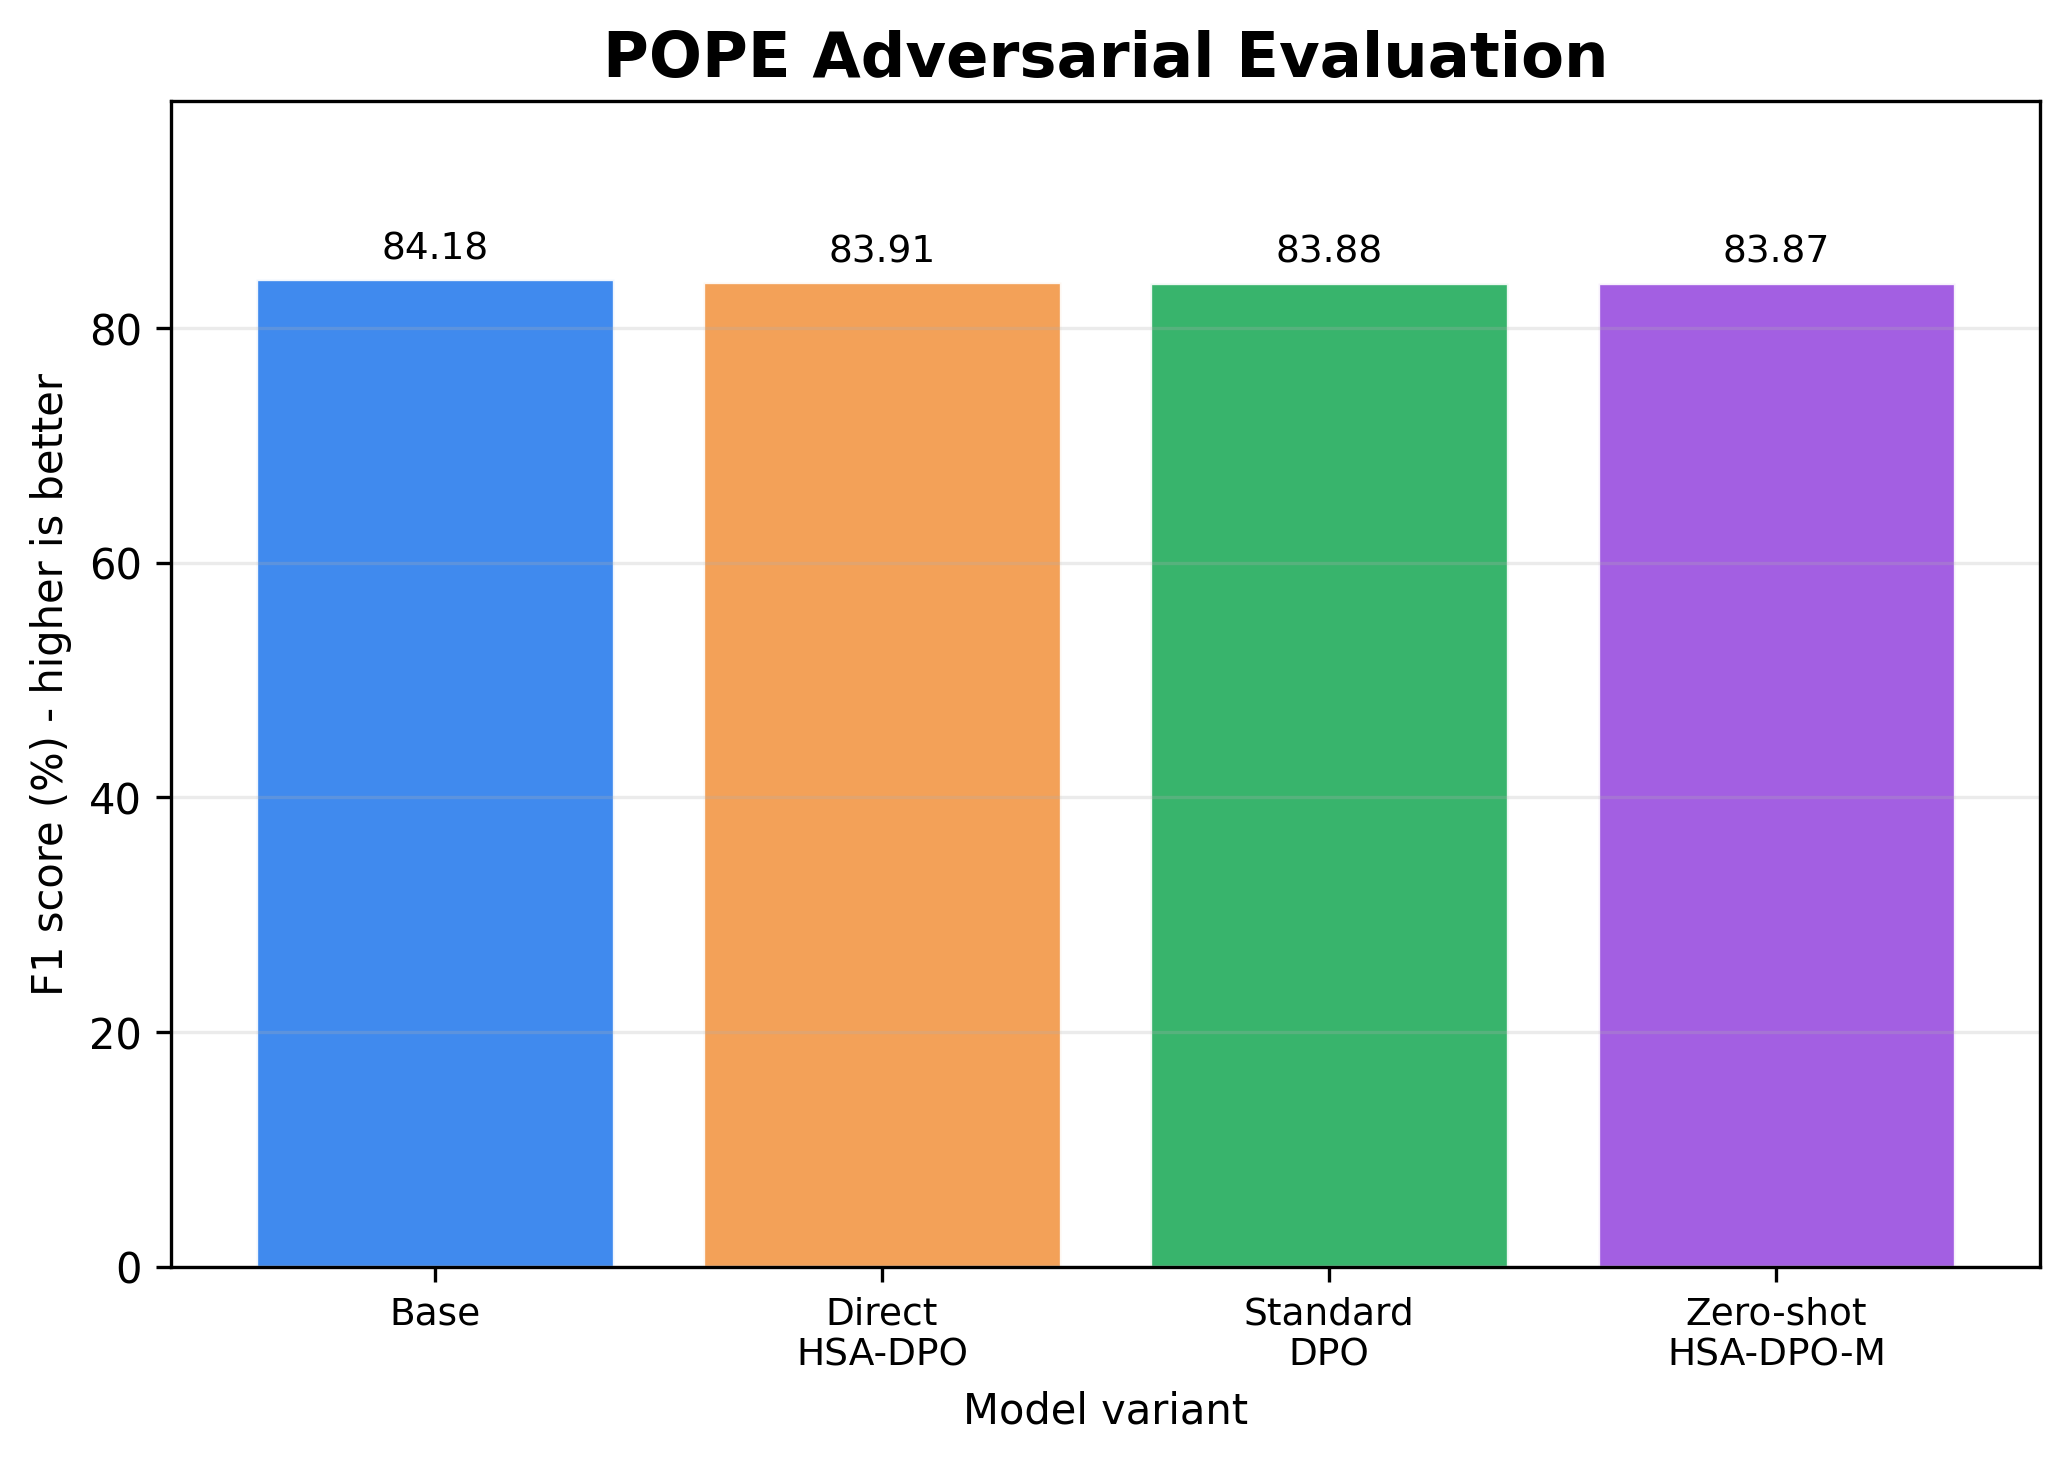
\includegraphics[width=0.48\linewidth,height=0.16\textheight,keepaspectratio]{../result_figures/pope_benchmark_histogram.png}
  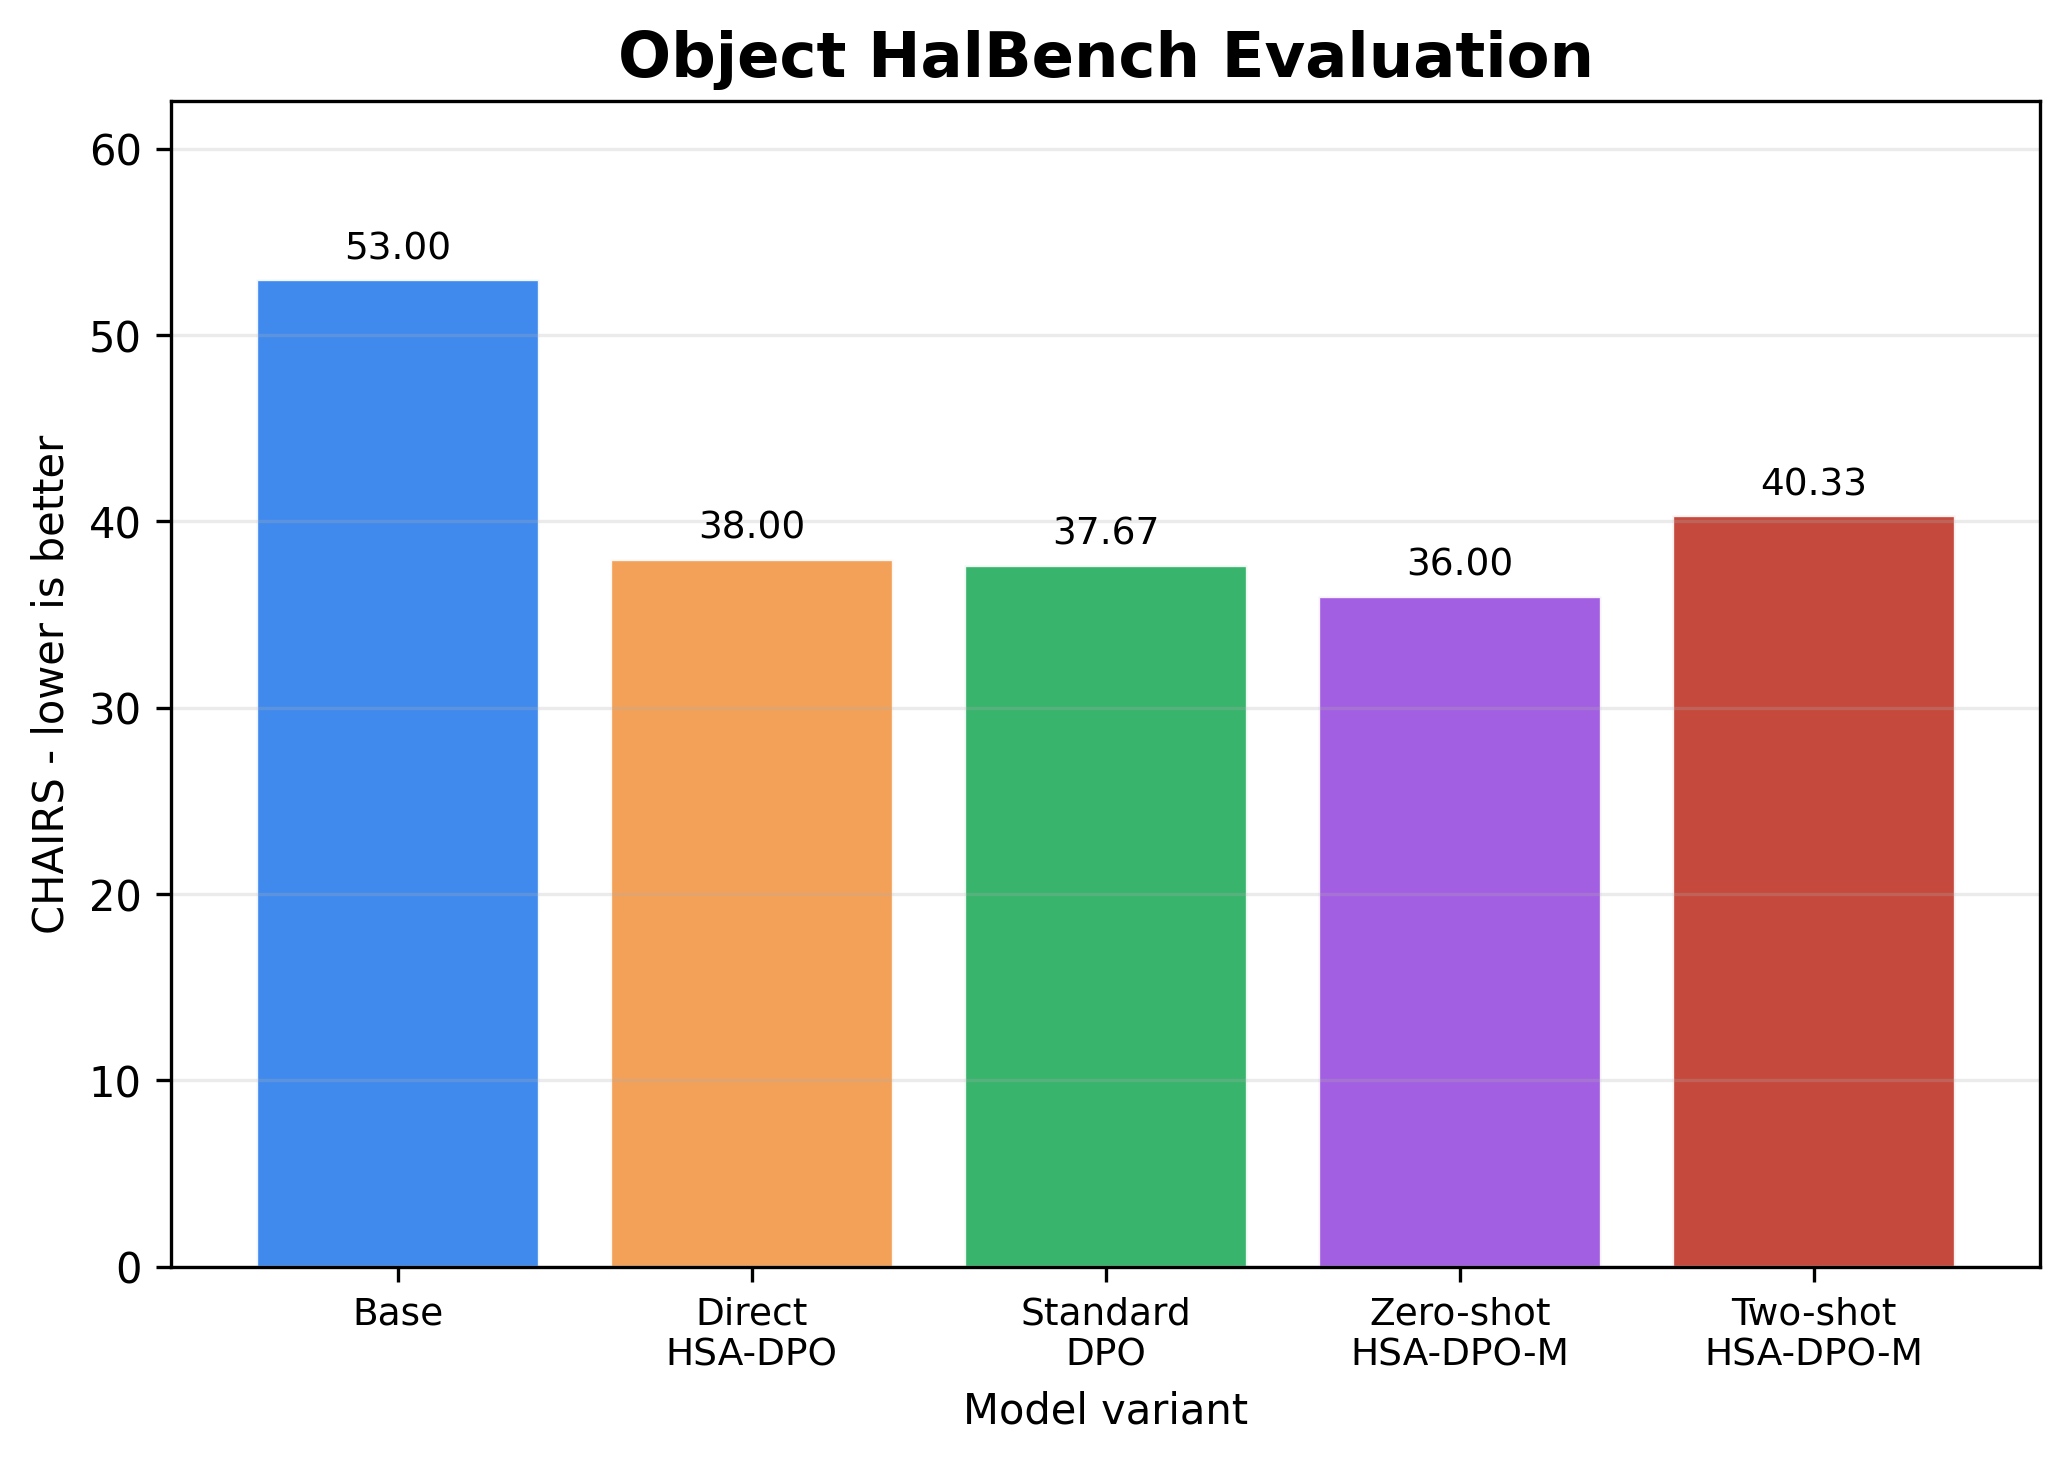
\includegraphics[width=0.48\linewidth,height=0.16\textheight,keepaspectratio]{../result_figures/object_halbench_histogram.png}\\[0.5em]
  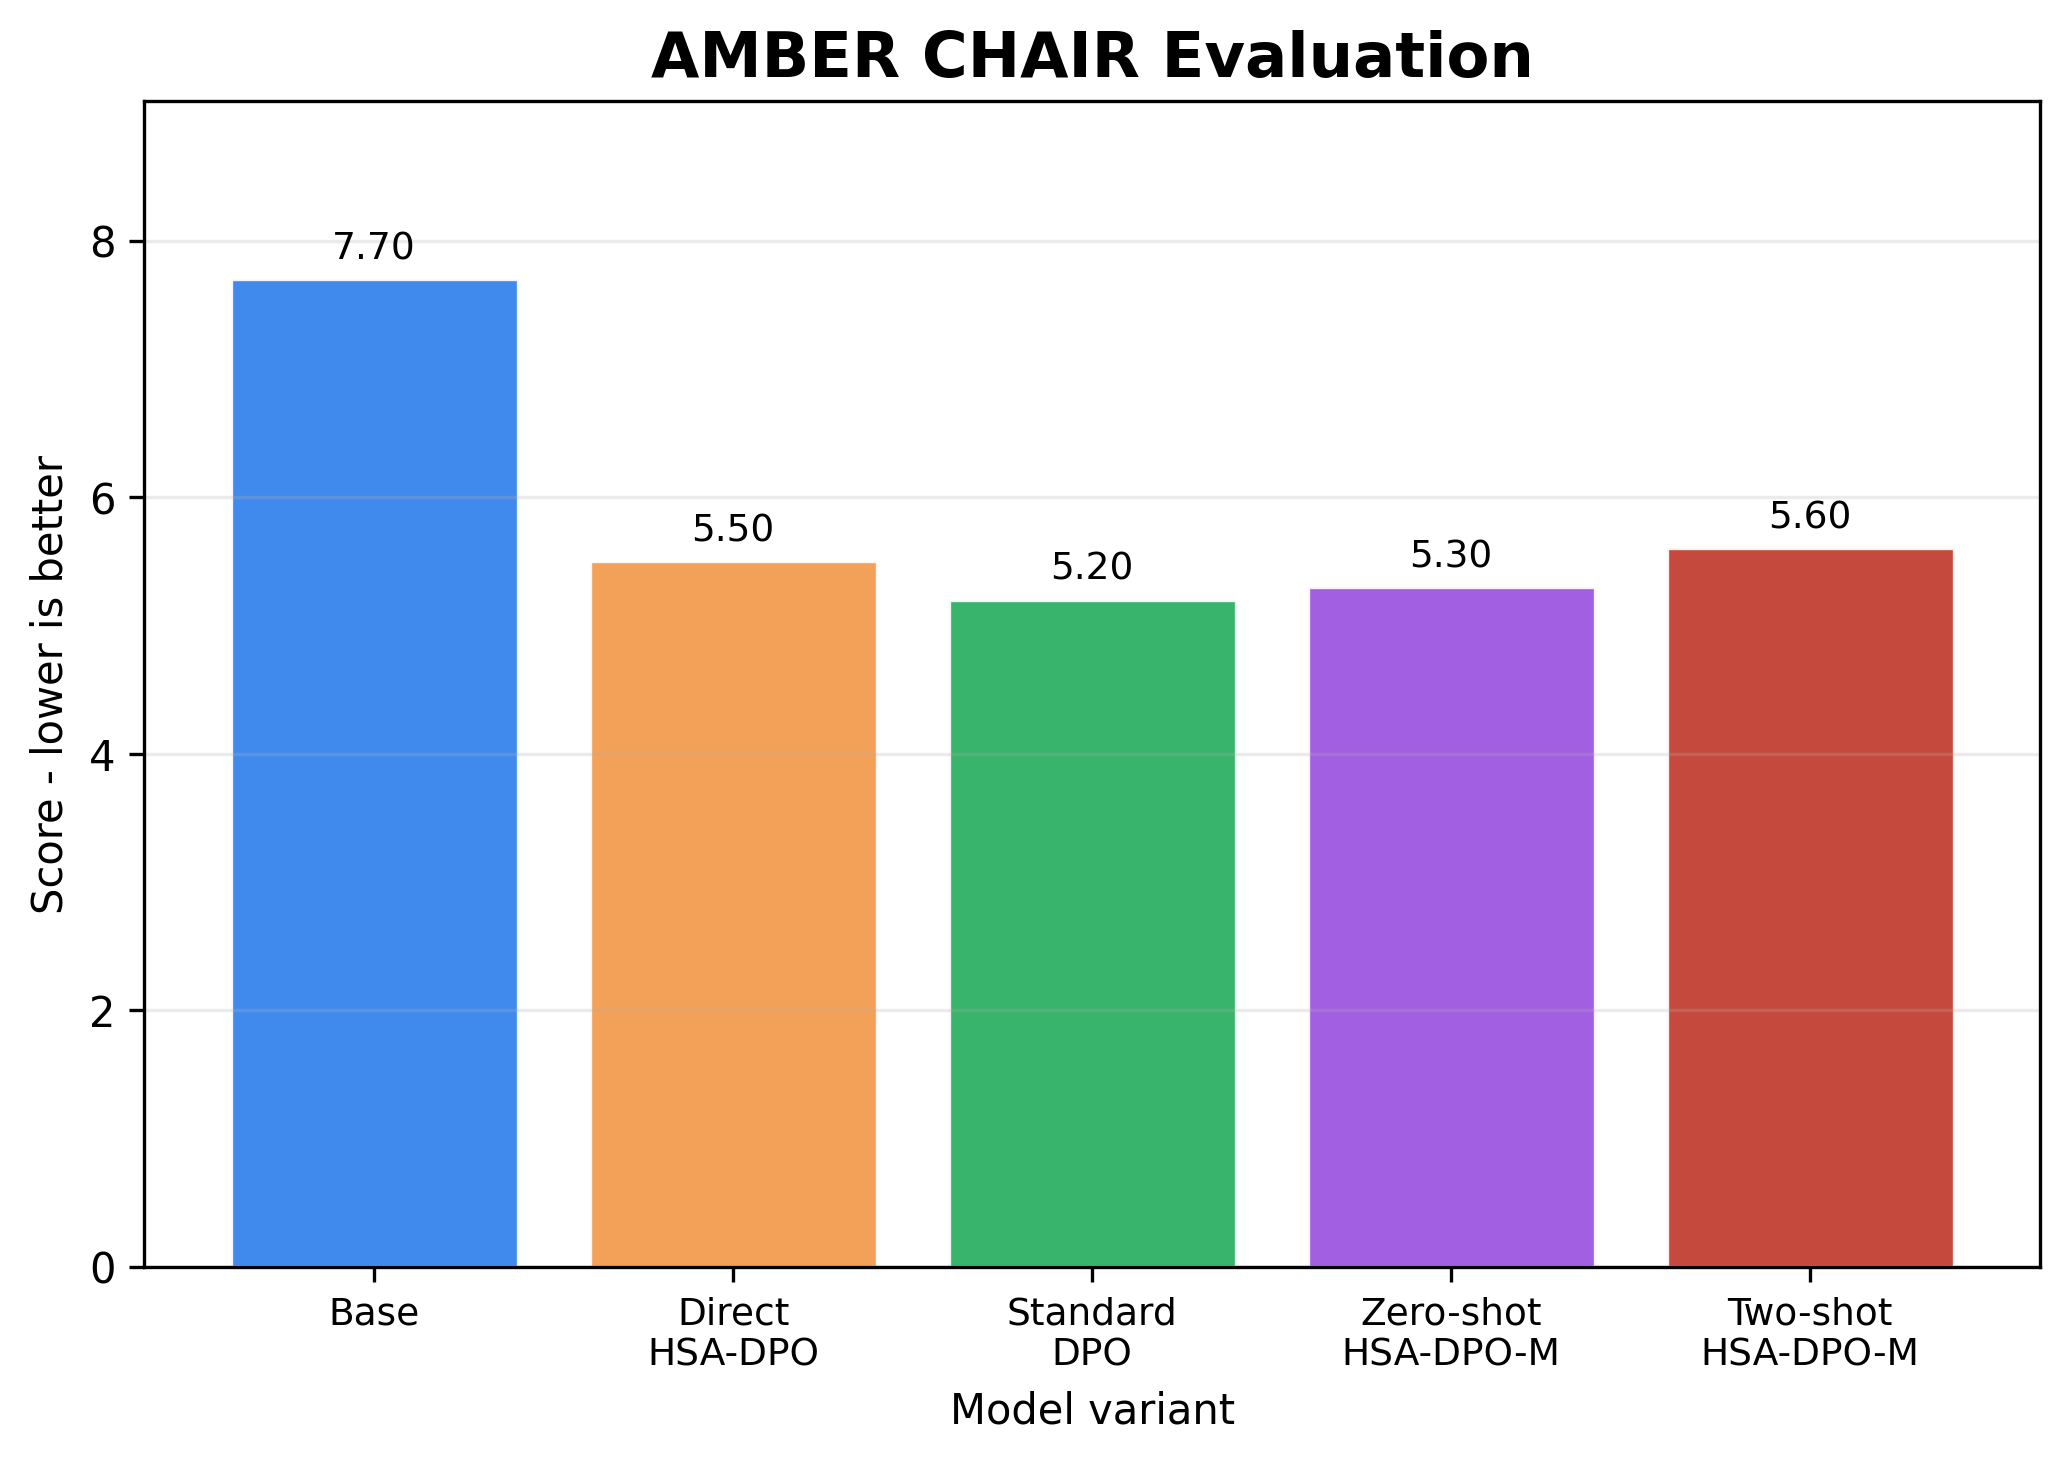
\includegraphics[width=0.48\linewidth,height=0.16\textheight,keepaspectratio]{../result_figures/amber_chair_histogram.png}
  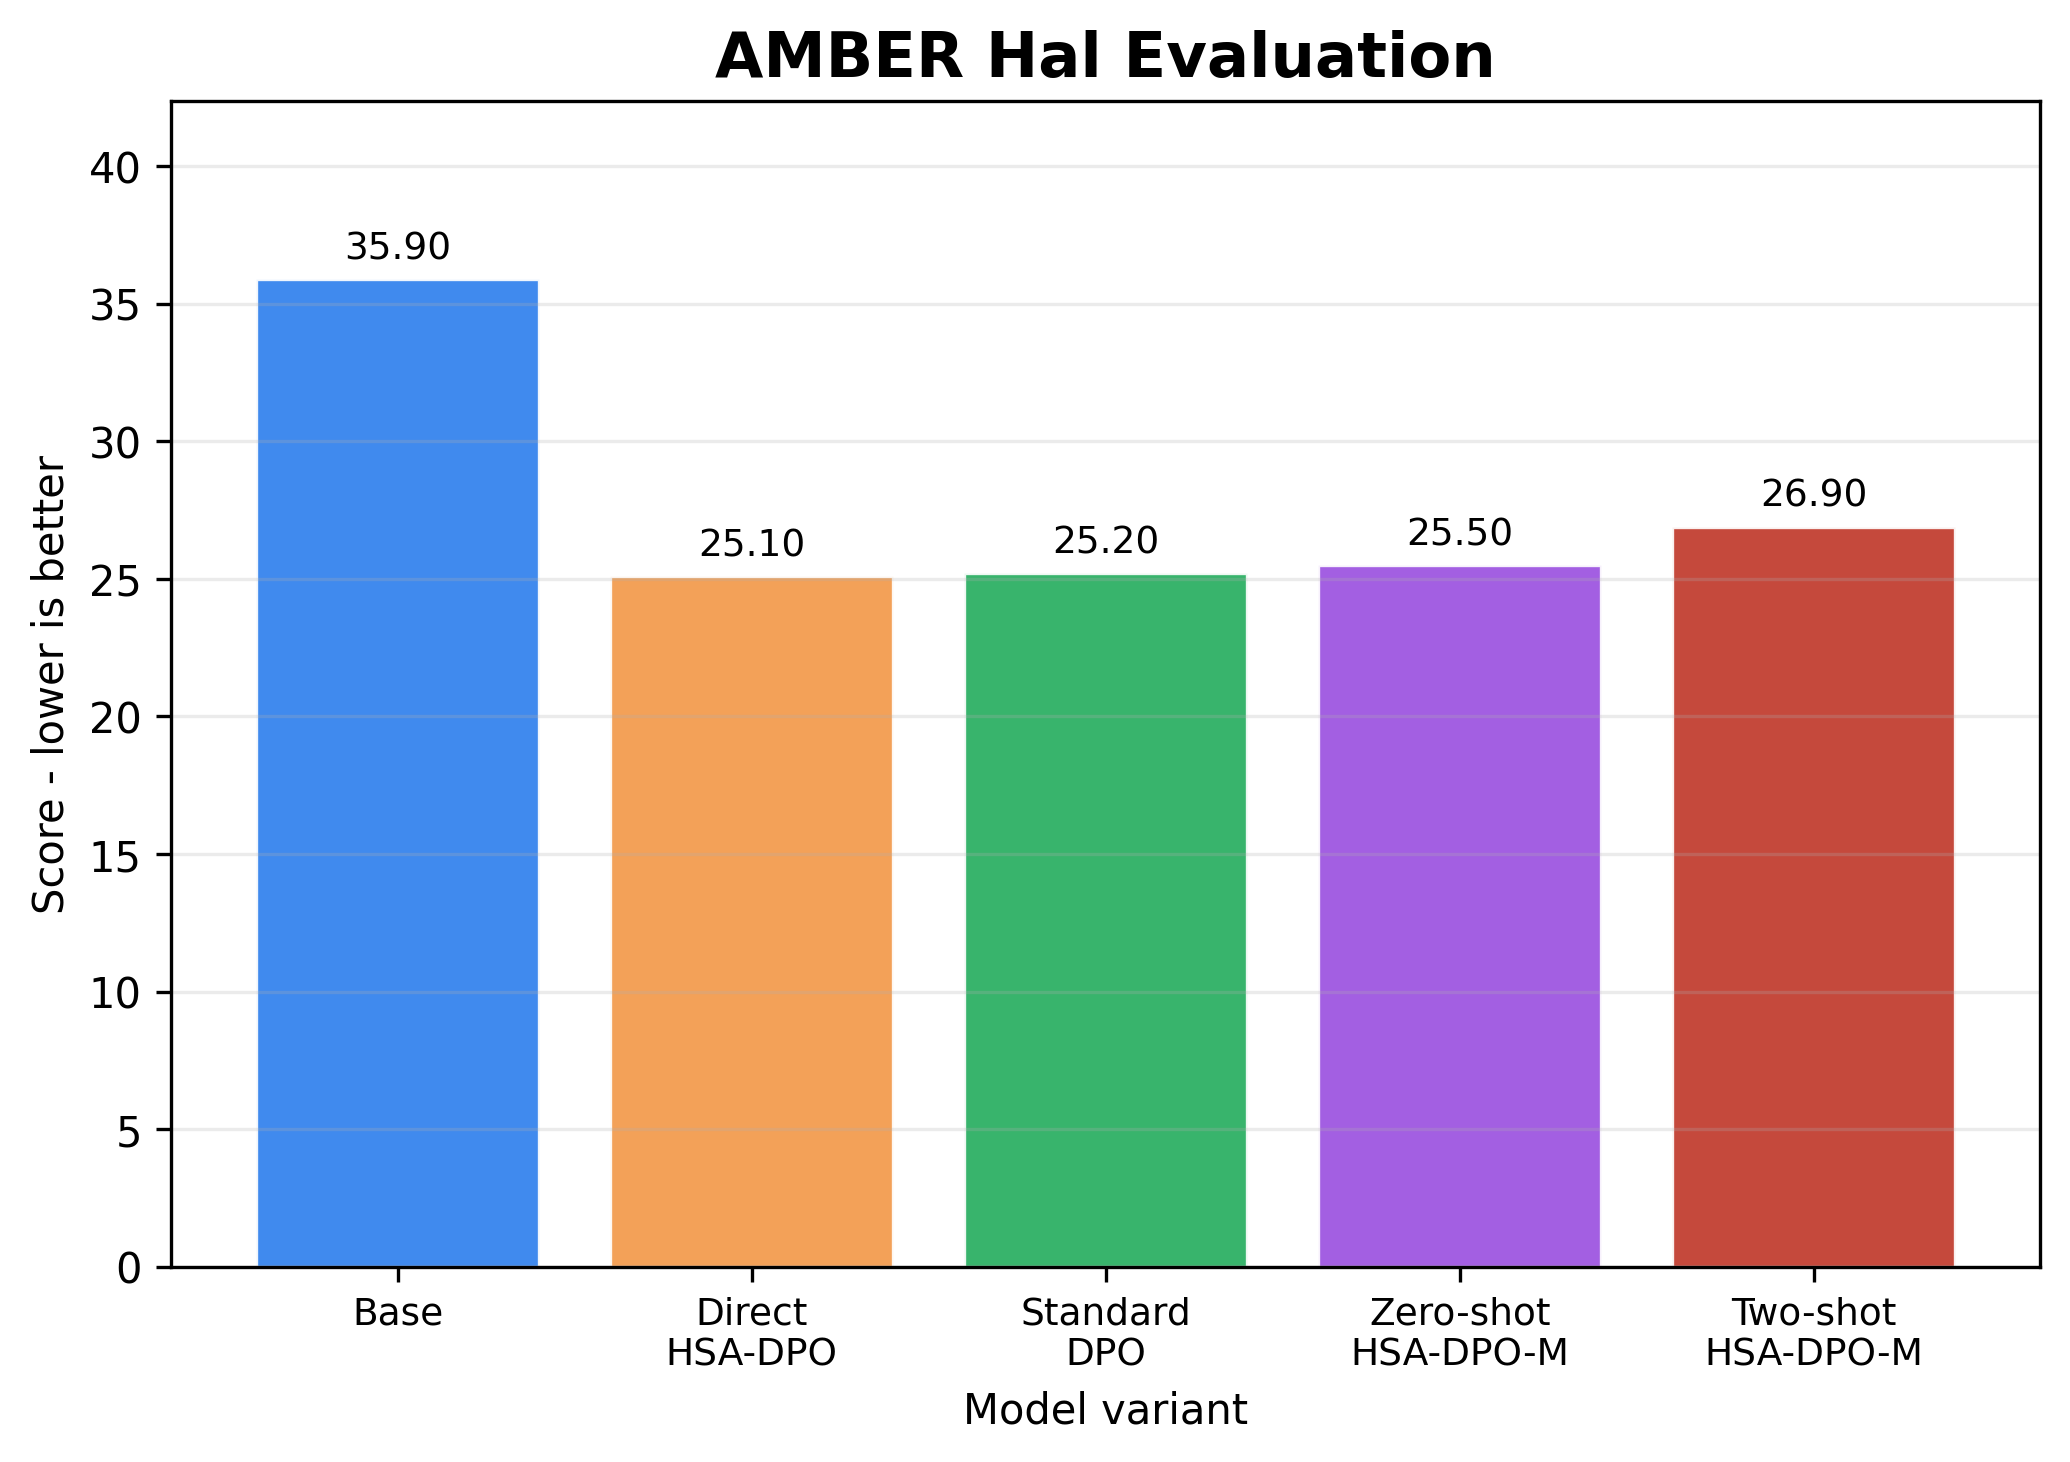
\includegraphics[width=0.48\linewidth,height=0.16\textheight,keepaspectratio]{../result_figures/amber_hal_histogram.png}
  \caption{Benchmark summaries for POPE, Object HalBench, AMBER-CHAIR, and AMBER-Hal. Results show limited POPE improvement but stronger reductions on Object HalBench and AMBER. The two-shot HSA-DPO-M variant is omitted from POPE because valid F1/recall values were unavailable.}
  \label{fig:benchmark-histograms}
\end{figure}


\section{Discussion}

The results show that fine-grained hallucination mitigation should not be evaluated as a single uniform improvement claim. The strongest gains appear on generative hallucination metrics, where the training signal is well aligned with the objective of removing unsupported content from free-form responses. Object HalBench and AMBER both reward reductions in hallucinated object mentions and unsupported visual claims, and these are exactly the types of errors targeted by the critique-guided preference data. The large decrease in Object HalBench CHAIRs and AMBER-Hal therefore supports the value of using fine-grained hallucination feedback as preference supervision.

At the same time, POPE reveals an important limitation. POPE adversarial evaluation is a binary object-presence setting, and the trained models become more precise but less recall-oriented. In practical terms, the models are less likely to answer positively when uncertain, which can reduce false positives but increase false negatives. This behavior is consistent with a mitigation pipeline that penalizes hallucination: the model learns caution. However, caution is not always equivalent to better benchmark performance, especially when recall is important. This explains why POPE F1 does not improve even though Object HalBench and AMBER hallucination metrics improve.

The comparison between standard DPO, direct HSA-DPO, zero-shot judged severity-margin HSA-DPO-M, and two-shot judged severity-margin HSA-DPO-M also suggests that severity information is useful, but not sufficient by itself. The zero-shot judged severity-margin variant obtains the best Object HalBench scores, while standard DPO is slightly better on AMBER-CHAIR and direct HSA-DPO is slightly better on AMBER-Hal. The two-shot judged run accepts fewer direct pairs, repairs more rejected pairs, and still improves over the base model on Object HalBench and AMBER, but it does not improve over the zero-shot judged variant. These differences indicate that the quality and distribution of preference pairs may matter as much as the exact severity-aware objective. In particular, judged validation can remove or repair weak pairs, but it can also reduce the amount and diversity of training data. A robust future version of the pipeline should therefore treat preference validation as a data-quality tradeoff rather than assuming that stricter filtering or few-shot prompting always improves downstream behavior.

The results answer the three research questions in a qualified way. For \textbf{RQ1}, the released annotations can be converted into structured critique and preference artifacts: the pipeline normalizes $16{,}143$ feedback records and uses $8{,}386$ released preference pairs for alignment experiments. For \textbf{RQ2}, judged validation and repair improve the inspectability of preference construction and recover some initially rejected examples, but the downstream effect is mixed. The zero-shot judged path keeps $8{,}062$ final verified pairs, while the two-shot judged path keeps $7{,}878$ final verified pairs; however, the two-shot variant does not outperform the zero-shot variant on the reported hallucination metrics. For \textbf{RQ3}, severity-aware DPO reduces hallucination in generative settings but not universally. Object HalBench CHAIRs drops from $53.00$ for the base model to $36.00$ for the best judged severity-margin run, and AMBER-Hal drops from $35.90$ to the $25.10$--$26.90$ range across trained variants. In contrast, POPE adversarial F1 remains slightly higher for the base model, so the answer is benchmark-dependent rather than a uniform yes.

Overall, the evidence supports a measured conclusion: fine-grained critique extraction and severity-aware alignment are useful tools for hallucination mitigation, especially for open-ended generation, but they do not automatically dominate simpler baselines across every benchmark. The most defensible interpretation is that the pipeline improves hallucination-specific generative behavior while introducing a conservative response tendency that must be managed when evaluating binary visual question settings.


\section{Limitations}

Our project has several limitations. First, it is primarily an implementation and reproduction effort rather than a fully novel hallucination mitigation framework. Second, the effectiveness of the full pipeline depends on the quality of the intermediate stages, especially critique extraction, rewriting, and preference validation. Third, due to project time constraints, not all benchmark settings or large-scale training runs have yet been completed. Finally, judged validation and repair decisions may be sensitive to the chosen evaluator, prompt, model checkpoint, and dataset, which means that observed behavior may vary across models and benchmarks.

\section{Conclusion}

This work implemented and evaluated a fine-grained hallucination mitigation pipeline for LVLMs. The pipeline normalizes released hallucination supervision into structured critiques, uses those critiques to support preference construction and repair, and trains LLaVA adapters with standard DPO, direct HSA-DPO, zero-shot judged severity-margin HSA-DPO-M, and two-shot judged severity-margin HSA-DPO-M objectives. The experimental results show that the approach is most effective on generative hallucination metrics: Object HalBench CHAIRs and AMBER hallucination scores decrease substantially compared with the base model. However, POPE adversarial F1 does not improve for the trained variants with valid POPE values, and the two-shot POPE artifact does not provide a valid F1/recall value.

The main conclusion is therefore not that severity-aware preference optimization universally improves LVLM hallucination behavior, but that fine-grained critique supervision provides a useful and inspectable training signal when it is aligned with the evaluation setting. Severity-aware methods can reduce unsupported visual content, especially in open-ended responses, but their success depends on the quality of preference pairs, the strictness of validation, and the benchmark objective. Future work should improve the judged-repair path, evaluate larger and more diverse LVLM backbones, and study how to preserve visual coverage while reducing hallucination.

\begin{ack}
This project was self-funded. The total project cost, including rented GPU compute and hosted API usage for preference validation, repair verification, training, and evaluation, exceeded USD 120.
\end{ack}

\bibliographystyle{plainnat}
\bibliography{references}

\appendix

\section{Prompt Templates}
\label{app:prompts}

This appendix records the prompt families used in the implementation. The released fine-grained annotations are treated as the main supervision source. The annotation-style prompts below are included to make the pipeline reproducible and to align the implementation with the fine-grained feedback and rewrite protocol used by HSA-DPO-style work \citep{xiao2025hsa}. No API keys or private credentials are included in any prompt template.

\subsection{Severity Rubric}
\label{app:severity-rubric}

All critique, detector, rewrite, and preference-construction stages use the same three-level severity convention. The score is later aggregated into a response-level severity value for severity-aware preference optimization.

\begin{quote}
\small
\textbf{Severity rubric.}
Minor (1 point): localized visual error that does not alter the main scene understanding.
Moderate (2 points): noticeable object, attribute, or relation error that changes part of the scene.
Major (3 points): central object, count, action, or relation error that substantially changes the answer.
Use only Minor, Moderate, or Major.
\end{quote}

\subsection{DDG Fine-Grained Annotation Prompt}
\label{app:ddg-prompt}

The DDG prompt is used for detailed-description style examples. It conditions the annotation on image-region information and the generated description. Its purpose is to produce sentence-level hallucination feedback, reasons, severity scores, and a corrected description.

\begin{quote}
\small
\textbf{Task instructions.}
You are tasked with evaluating the accuracy of a detailed description of an image against provided Visual Genome regions. Identify hallucinated object, attribute, and relationship claims, explain why they are hallucinations, assign severity scores, and provide a corrected rewritten description.

\textbf{Severity rubric.}
Use the Minor, Moderate, Major rubric from Appendix~\ref{app:severity-rubric}.

\textbf{Image Regions Information:}
\texttt{\{regions\}}

\textbf{Description:}
\texttt{\{description\}}

\textbf{Output Format:}
Tagged Description;
Reasons;
Scores;
Rewritten Description.
\end{quote}

\subsection{VCR Fine-Grained Annotation Prompt}
\label{app:vcr-prompt}

The VCR prompt is used for visual complex reasoning examples. It asks the annotator to inspect a reasoning answer, identify hallucinated object, attribute, or relationship claims, assign severity, and return a corrected answer. The prompt limits the number of tagged hallucination sentences to keep the feedback focused.

\begin{quote}
\small
\textbf{Task instructions.}
You are tasked with evaluating the accuracy of a complex reasoning answer for an image. Identify hallucinated object, attribute, and relationship claims, explain why they are hallucinations, assign severity scores, and provide a corrected rewritten answer. Do not tag more than three hallucination sentences.

\textbf{Severity rubric.}
Use the Minor, Moderate, Major rubric from Appendix~\ref{app:severity-rubric}.

\textbf{Complex reasoning:}
\texttt{\{reasoning\}}

\textbf{Output Format:}
Question and Tagged Answer;
Reasons;
Scores;
Rewritten Answer.
\end{quote}

\subsection{Local Detector Prompt}
\label{app:detector-prompt}

The detector-style prompt is used when a local LVLM is asked to produce fine-grained hallucination findings from an image, task context, and candidate response. The model must either return a structured Tags/Scores report or exactly state that no hallucination is present.

\begin{quote}
\small
You are a fine-grained hallucination detector for a vision-language model. Given an image and a candidate response, return exactly one of these formats:

\textbf{1.} \texttt{NO HALLUCINATION}

\textbf{2.} A Tags/Scores report matching this structure:

\textbf{Tags:}
\texttt{<object>} hallucinated object claims;
\texttt{<attribute>} hallucinated attribute claims;
\texttt{<relationship>} hallucinated relationship claims.

\textbf{Scores:}
For each tagged claim, provide the evidence span, severity label, numeric severity score, and concise visual rationale.

\textbf{Rules.}
Use only object, attribute, and relationship types. Use only Minor, Moderate, or Major. If there is no hallucination, return \texttt{NO HALLUCINATION} exactly. Do not add extra commentary before or after the required output.

\textbf{Prompt or task context:}
\texttt{\{question\}}

\textbf{Candidate response to assess:}
\texttt{\{response\}}
\end{quote}

\subsection{Critique-Guided Rewrite Prompt}
\label{app:rewrite-prompt}

The rewrite prompt is used by LLaVA to convert a hallucinated response into the chosen response of a preference pair. The prompt receives the original response and the fine-grained critiques. It asks the rewriter to remove unsupported content while preserving visually supported details. This is the prompt family used for the main critique-guided rewrite stage.

\begin{quote}
\small
You are rewriting a hallucinated vision-language response for the fine-grained hallucination mitigation pipeline. Use the image and verified critiques to produce the preferred answer.

\textbf{Question or task context:}
\texttt{\{question\}}

\textbf{Original response:}
\texttt{\{original response\}}

\textbf{Detected hallucination tags and reasons:}
\texttt{\{critiques with type, severity, evidence, and rationale\}}

\textbf{Instructions.}
The tags may not always be correct; rely on the image and remove only unsupported claims. Correct or remove every identified hallucination. Preserve accurate visual content from the original response. Do not add unsupported objects, attributes, relations, counts, actions, or identities. Output only the rewritten answer.
\end{quote}

\subsection{Released-Preference Validation Prompt for Gemini and GPT}
\label{app:api-validation-prompt}

The judged-preference path uses hosted VLM judges to validate released preference pairs. Gemini and GPT receive the same text prompt and the corresponding image. The judges do not rewrite the answer; they only decide whether the chosen response is a reliable improvement over the rejected response. The implementation can run either a single judge or both judges. When both are used, the decision rule can be configured as either accepting when at least one judge approves or accepting only when both approve. In the zero-shot experiment, the target pair is presented directly after the rubric. In the two-shot experiment, the calibration block in Appendix~\ref{app:two-shot-validation-prompt} is inserted before the target pair.

\begin{quote}
\small
You are validating a hallucination-mitigation preference pair for a vision-language model. Use the image as the source of truth. Return exactly one JSON object and no other text. The JSON object must have exactly these keys: \texttt{approved}, \texttt{reason}. \texttt{approved} must be a JSON boolean. \texttt{reason} must be one concise sentence.

Approve when the chosen rewrite clearly improves factual visual grounding over the rejected response, removes or reduces the tagged hallucination, and does not introduce a new important hallucination. Reject when the chosen rewrite is still unsupported by the image, loses essential correct content, or is not clearly better than the rejected response. Be conservative, but do not reject only because the chosen response is shorter.

\textbf{Question:}
\texttt{\{question\}}

\textbf{Rejected/original response:}
\texttt{\{rejected response\}}

\textbf{Chosen/rewrite response:}
\texttt{\{chosen response\}}

\textbf{Original hallucination tags and severity:}
\texttt{\{rejected tag text\}}

Return only the JSON object now.
\end{quote}

\subsection{Two-Shot Validation Calibration Block}
\label{app:two-shot-validation-prompt}

The two-shot experiment uses the same validation prompt as Appendix~\ref{app:api-validation-prompt}, but inserts two text-only calibration examples before the target pair. These examples teach the approval rule without claiming that their visual details are present in the target image.

\begin{quote}
\small
Two calibration examples follow. They are text-only examples for the decision rubric; do not assume their visual details are present in the target image.

\textbf{Example 1.}

\textbf{Question:}
Describe the image.

\textbf{Rejected/original response:}
The image shows a child holding a red umbrella while a dog walks nearby.

\textbf{Chosen/rewrite response:}
The image shows a child holding an umbrella.

\textbf{Original hallucination tags and severity:}
object hallucination: dog nearby; attribute hallucination: red umbrella; severity major

\textbf{Expected JSON:}
\texttt{\{"approved": true, "reason": "The chosen response removes the unsupported dog and color claims while preserving the grounded umbrella detail."\}}

\textbf{Example 2.}

\textbf{Question:}
What is happening in the scene?

\textbf{Rejected/original response:}
A man is sitting on a bench with a bicycle beside him.

\textbf{Chosen/rewrite response:}
A man is sitting on a bench beside a motorcycle in a park.

\textbf{Original hallucination tags and severity:}
object hallucination: bicycle beside him; severity moderate

\textbf{Expected JSON:}
\texttt{\{"approved": false, "reason": "The chosen response introduces unsupported motorcycle and park details, so it is not a reliable improvement."\}}
\end{quote}

\subsection{API Critic Feedback Prompt}
\label{app:api-critic-prompt}

For the optional judged-repair path, Gemini or GPT can be used as a critic after an initial LLaVA rewrite. In this setting, the hosted VLM is explicitly restricted to feedback only. It should identify remaining hallucinations, unsupported additions, removed correct details, or over-editing, but it should not write the final answer.

\begin{quote}
\small
You are a critic for a hallucination-mitigation rewrite of a vision-language response. Your job is to provide feedback only. Do not write the final answer.

\textbf{Question or task context:}
\texttt{\{question\}}

\textbf{Original response:}
\texttt{\{original response\}}

\textbf{Detected hallucination tags and reasons from the local detector:}
\texttt{\{detected critiques\}}

\textbf{Initial rewritten response:}
\texttt{\{initial rewrite\}}

Check the initial rewrite against the image and detector findings. Return concise feedback about remaining hallucinations, unsupported additions, removed correct details, or over-edits. If the rewrite is acceptable, return exactly: \texttt{NO CRITICAL ISSUES}. Do not provide a replacement answer. Do not use markdown tables.
\end{quote}

\subsection{Feedback-Guided Revision Prompt}
\label{app:revision-prompt}

The feedback-guided revision prompt is used when LLaVA receives the original response, critique information, the initial rewrite, and critic feedback. Unlike the critic prompt, this prompt produces the final repaired answer.

\begin{quote}
\small
You are revising a hallucination-mitigation rewrite for the final preference pair. Use the image, local detector findings, the initial rewrite, and critic feedback.

\textbf{Question or task context:}
\texttt{\{question\}}

\textbf{Original response:}
\texttt{\{original response\}}

\textbf{Detected hallucination tags and reasons:}
\texttt{\{detected critiques\}}

\textbf{Initial rewritten response:}
\texttt{\{initial rewrite\}}

\textbf{Critic feedback:}
\texttt{\{critic feedback\}}

\textbf{Instructions.}
The detector and critic feedback may be wrong; rely on the image. Remove unsupported claims and preserve correct supported details. Do not add unsupported objects, attributes, relations, counts, actions, or identities. Output only the final revised answer.
\end{quote}

\subsection{Rejected-Pair Repair Prompt}
\label{app:repair-prompt}

When a preference pair fails validation, LLaVA can repair the chosen response. The repair prompt uses the original rejected response, the current chosen rewrite, the fine-grained critiques, and the validation reasons from the judges. The rejected response remains fixed; only the chosen response is repaired.

\begin{quote}
\small
You are repairing a hallucination-mitigation rewrite for a vision-language model.

Use the image as the source of truth. Produce only the final corrected answer, with no markdown and no explanation.

The current chosen rewrite was rejected by the API judges. Revise it so it is better grounded in the image, preserves correct useful details, removes unsupported details, and avoids adding new unsupported claims.

\textbf{Question:}
\texttt{\{question\}}

\textbf{Original rejected response:}
\texttt{\{rejected response\}}

\textbf{Current chosen rewrite:}
\texttt{\{chosen response\}}

\textbf{Original hallucination tags and severity:}
\texttt{\{rejected tag text\}}

\textbf{API judge feedback:}
\texttt{\{judge votes and reasons\}}

\textbf{Final corrected answer:}
\end{quote}

\subsection{Repaired-Pair Verification Prompt}
\label{app:repair-verify-prompt}

After LLaVA repair, the validation prompt in Appendix~\ref{app:api-validation-prompt} is reused to verify repaired pairs. In the two-shot experiment, GPT-4.1-mini uses the calibration block from Appendix~\ref{app:two-shot-validation-prompt}. The repaired answer is placed as $y^+$, the original hallucinated answer remains $y^-$, and the judge returns \texttt{\{"approved": true/false, "reason": "one concise sentence"\}}. Approved repairs are merged into the judged-preference training set; failed repairs are removed.

\end{document}
